\chapter{\label{chapter:Sandbox}The Sandbox}

\section{Design Principles}

\subsection{Sandbox Responsibilities}

\begin{enumerate}
\item Clones configured objects for use during a run.
\item Connects local objects and commands together during initialization.
\item Runs the Mission Control Sequence.
\item Responds to interrupts from teh Moderator.
\item Passes output data to the Publisher.
\item Coordinates mission-run communications with outside processes.
\item Resets itself for new runs.
\end{enumerate}

\section{Design}

\subsection{Class Details}

\subsubsection{Class Attributes}

\subsection{\label{section:SandboxLateBinding}The Late Binding Strategy}

\subsubsection{\label{section:SandboxInitialization}Sandbox Initialization Details}

Figure~\ref{figure:SequenceInit} shows the steps taken to initialize a control sequence -- either
the Mission Control Sequence or a Function Control Sequence.

\begin{figure}[htb]
\begin{center}
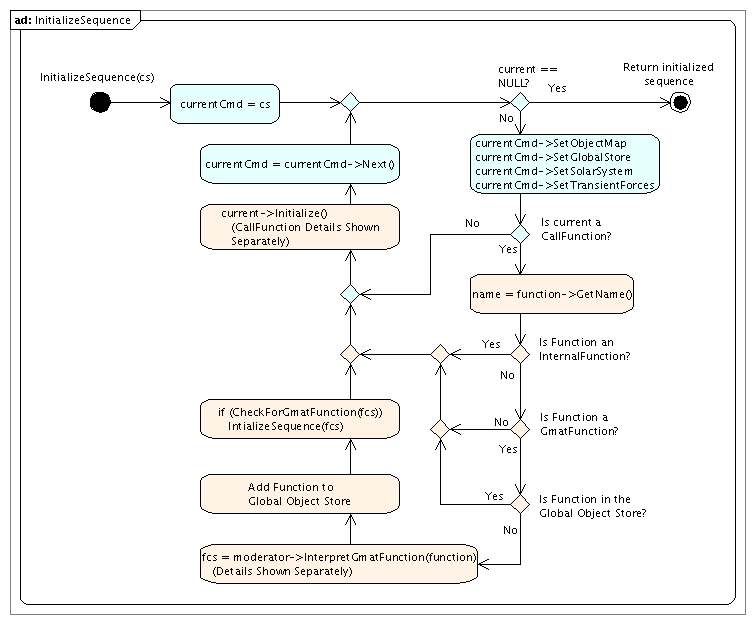
\includegraphics[378,312]{Images/InitializeSequence.png}
\caption{\label{figure:SequenceInit}Initialization of a Control Sequence in the Sandbox}
\end{center}
\end{figure}

\subsection{\label{section:SandboxInterruptPolling}Interrupt Polling During a Run}

\section{Usage and Modification}

